
\chapter{Design Decisions}
This chapter presents the decisions taken in this software project. The decisions are reasoned based on requirements from General Acoustics e.K. First the general requirements regarding the software are introduced, afterwards an overview of the architectural decisions is presented, and at last, implementation specific decisions including the selection of used libraries and programming environments are illustrated. 
\section{External Requirements}
The requirements from General Acoustics e.K. for this project were based on previous experiences with ADCP's as well as a glance into the future on forthcoming projects.\\ 
The requirements regarding the ADCP functionality were, (R1) the software should be able to parse real-time ADCP data on a low-power data logger, clean it by removing unused information and thus enable the possibility of logging longer time periods due to the reduced size. The other hard requirement was (R2) the possibility of processing old raw data files with focus on speed rater than efficiency. This implicitly required (R3) the application to scale according to the available hardware.\\ 
The requirements with an eye into the future also had a big impact on the development. One important aspect was (R4) portability. Unlike current software from General Acoustics e.K. the written code should be usable on low-power Linux or Windows IoT devices (e.g. RaspberryPi 3 \cite{raspberry} or BananaPro \cite{bananapro}) as well as on the Windows x96/x64 architecture. The decision was to go with C++ 11 \cite{cpp_11}, which offers portability, high efficiency and a native compiler for all platforms. The use of C++ as a high performance low-level programming language was also influenced by the requirement (R5) to save electricity, since e.g. the data logger has to run on battery for real-time operation. If the application needs fewer processing time, it also saves energy. \\
The application should be future-proof, on a short sight (R6) it should allow additional processing steps apart from the parsing. A viable option would be the addition of a wave analysis step. On a long-term view (R7) the architecture should allow other sensor types without having to change sensor unrelated code.

To benefit as much as possible from this software project, General Acoustics e.K. required to implement code parts that could be used for other applications as reusable and self contained as possible. These re-usability and extensibility requirements imply (R8) a well structured component based implementation approach. The components should be (R9) decoupled as much as possible. Reusable algorithms e.g. MATLAB related implementations, with no dependency to the ADCP context should be (R10) implemented as completely independent components.

The main efforts in this software project should be used for clear, simple, and correct algorithms framed in a well organized structure rather than building the perfect all-rounder. As an example, to make simple chaining of various components at runtime possible, one way would need to make the components persistent e.g. through an extensible markup language (XML) description. This would require the definition of a complex architecture, which only serves as the frame for the actual application. The implementation effort needed would exceed the scope of this project and move the focus from the implementation of the core algorithms to their frame. If needed such a frame could be implemented in a future project, and use the developed components from this software project. Nevertheless, the desired extensibility should be given, and may be implemented as simple \texttt{if-else} statements selecting the desired components in the main program.

To summarize the requirements of General Acoustics e.K., the application should
\begin{itemize}
\item parse and clean real-time ADCP data (R1), post-process old raw data (R2)
\item scale, depending on the hardware (R3),
\item be written in C++ for portability (R4) and efficiency (R5),
\item allow new functionality (R6, R7), and
\item be implemented in a component based approach (R8) where the components are as decoupled and independent as possible (R9, R10).
\end{itemize}
The development of a complete all-rounder to consider future scenarios is not a target of this project, but it should be easily extensible for additional components. Based on these requirements the following two sections highlight the design decisions taken in the development process. 

\section{Architectural Decisions}
The nature of the real-time parsing problem itself directs the architectural decisions. It can be seen as a pipelined input - process - output model. Each step in this pipeline represents one or a chain of components. It would be possible to implement the problem as one task in a script, probably saving a lot of development time, but in the end an inflexible monolith would have been created that disobeys every requirement from General Acoustics e.K. described above in Section 3.1.

The decision to proceed with a threaded approach to implement the pipeline was reasoned based on the following arguments: (1) A threaded approach works best if the functionality in each thread is completely unrelated and can run concurrently against the other threads, this is given, the input-, processing-, and output functionalities are independent. Each thread waits on data, and if it is finished doing its work it outputs the data to the next step. Another important aspect (2) is the really good scalability generated through the use of threads. If the application is run on a computer with a lot of processing power and many central processing unit (CPU) cores, each thread can run in parallel and speed up the execution. If it is running on a low-power single core processing unit it will execute the threads consecutively like it would be done in a monolithic way. The disadvantage would be the regular context switches between the threads. This disadvantage is more extreme on low-power devices with a low number of cores which are used for real-time processing, and here the processing time is by far fast enough.

A threaded approach would not be the only possibility to parallelize and scale the application, a task based approach with asynchronous nonblocking tasks would have worked in a similar way. Software currently produced at General Acoustics e.K., in general outsources input and output activities into threads to be sure that the software is able to e.g. read on a serial port continuously, other functionality in the software is handled in a task based way. If this approach would have been taken into account for this project two of three steps from the pipeline (input - processing - output) would already have been threads. To simplify and unify the use of components for all steps in regard to the requirements R6, R7, and R8, a completely threaded approach was chosen. Figure 3.1 shows a high level data flow diagram (DFD) of the three threads of the pipeline steps modeled as circles. The threads are connected over First-In-First-Out (FIFO) data structures represented as datastore objects. 

\begin{figure}[ht]
\centering
      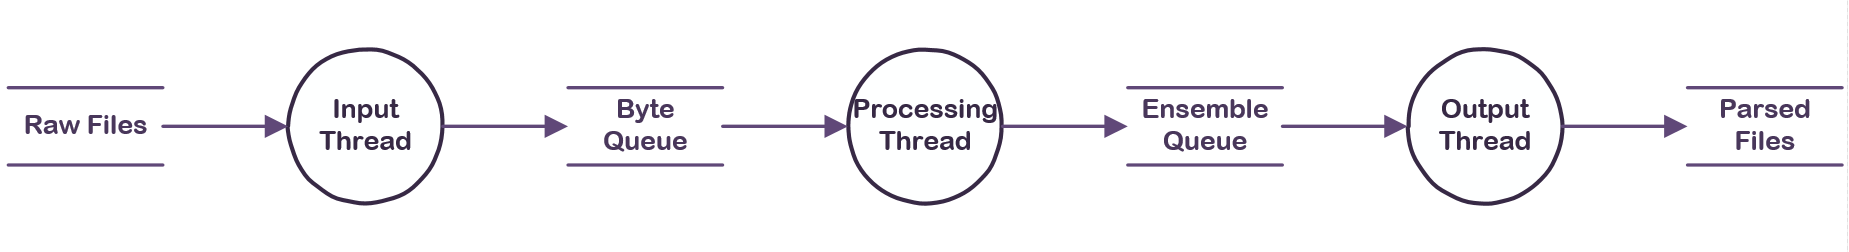
\includegraphics[width=1\textwidth]{dfd}
        \caption{A DFD showing the data-flow through the threads.}
\end{figure}

\begin{figure}[ht]
\centering
      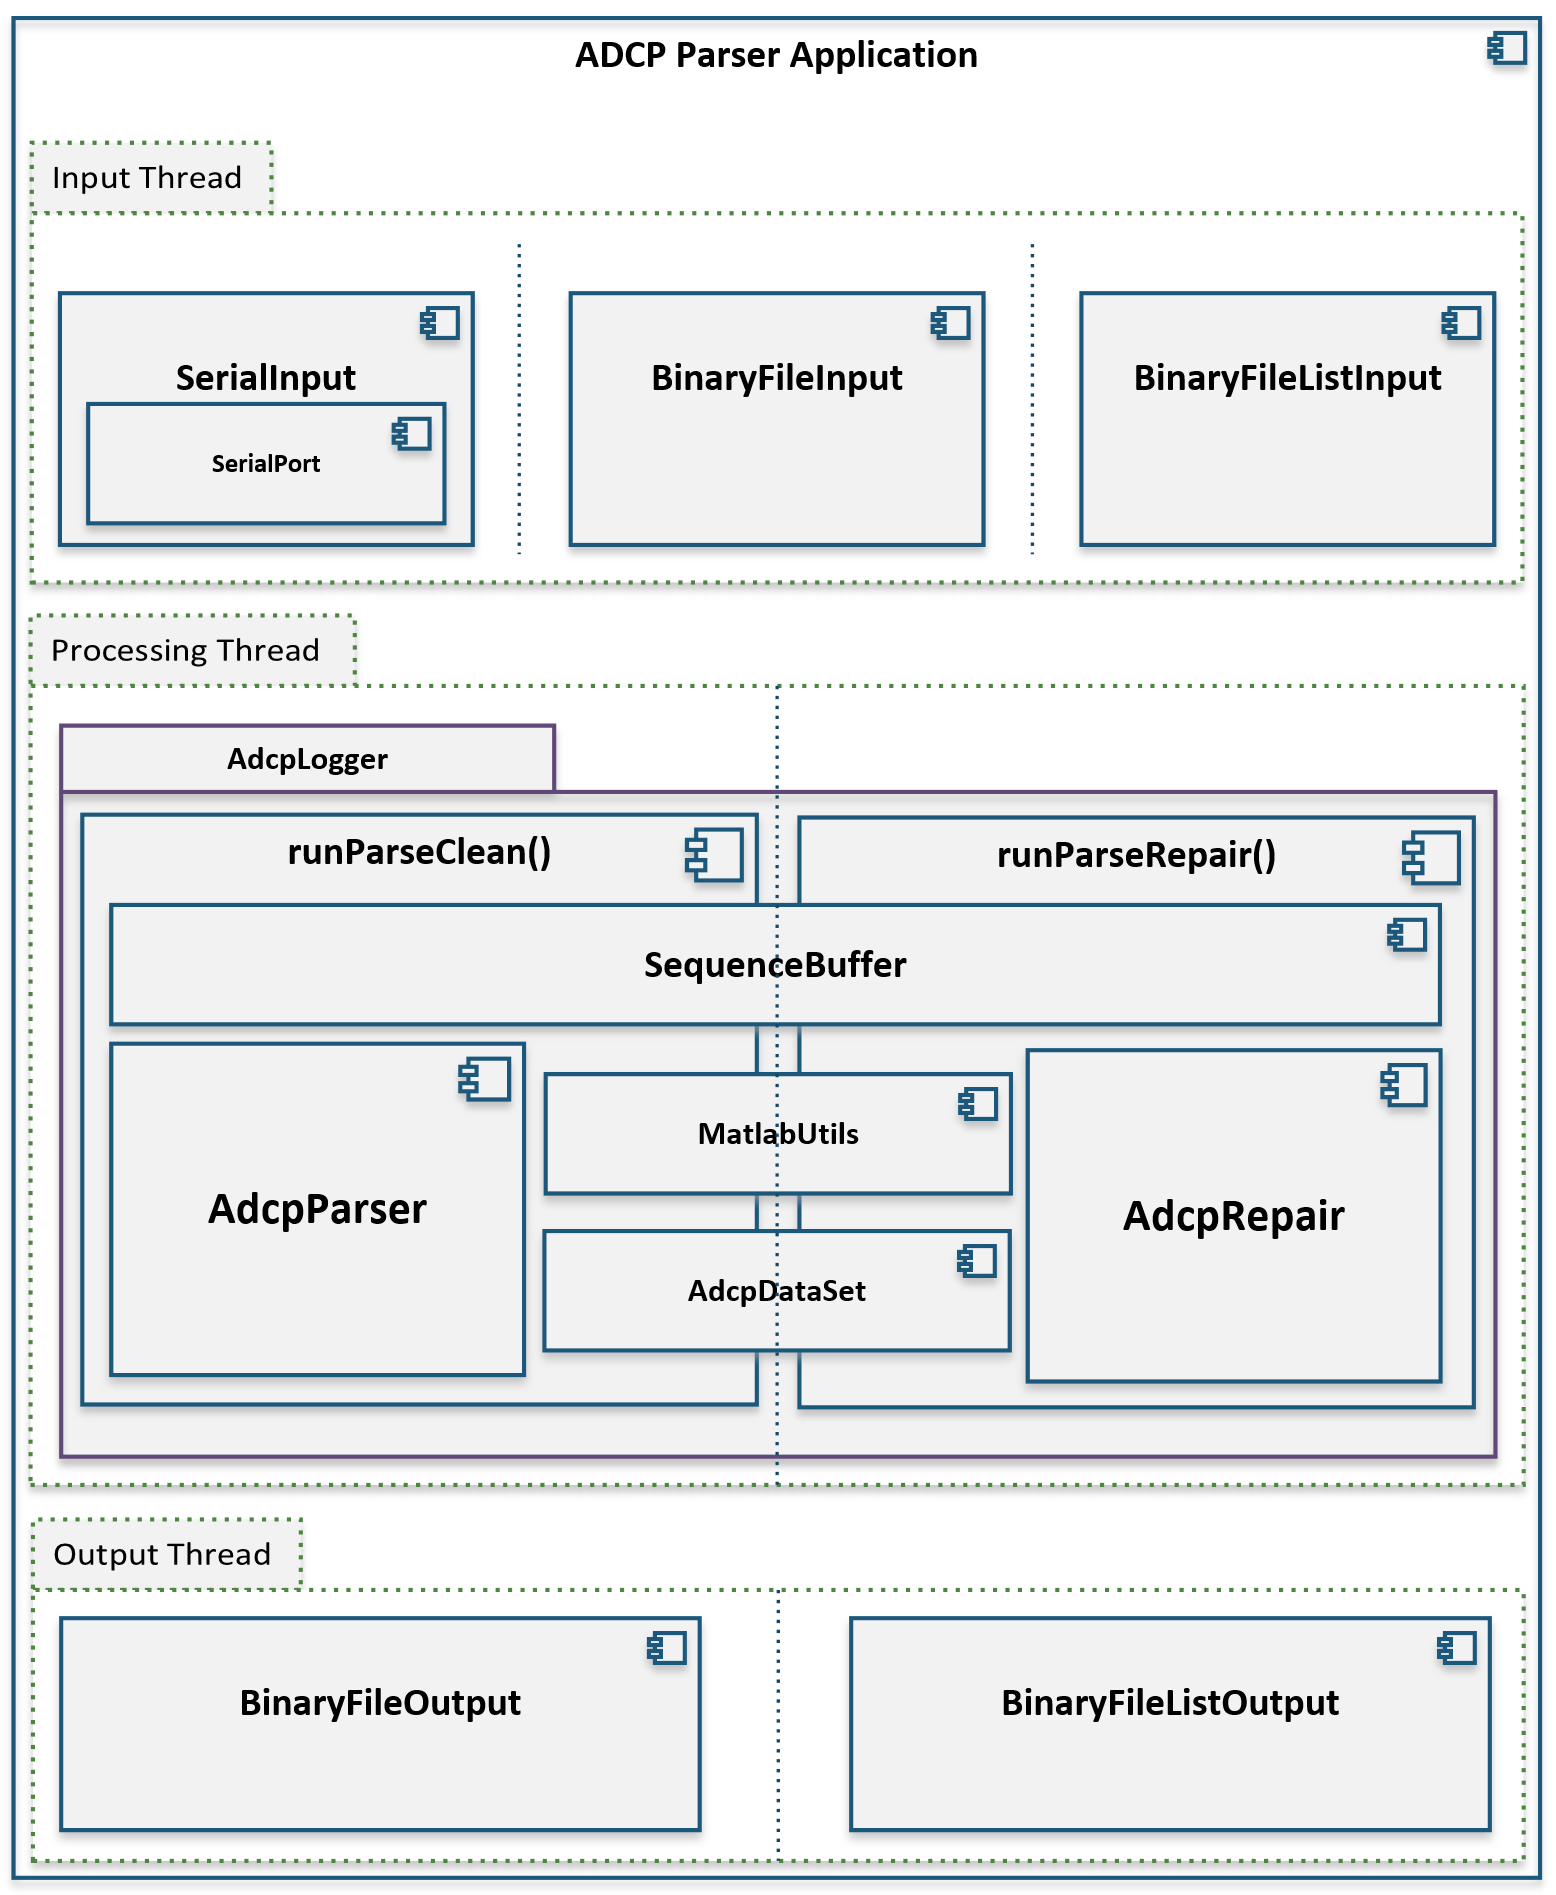
\includegraphics[width=0.8\textwidth]{all_components}
        \caption{Component diagram of the software}
\end{figure}

Figure 3.2 shows all components of the decided architecture in a component diagram, the threads may be viewed as unified modeling language (UML) packets with dashed lines. Dashed vertical lines signal a choice of components when the application is executed. If a component is used by other components it is drawn overlapping or completely inside of the using component. A component can be seen as a class or as a group of related classes, the exact implementation will be presented in Chapter 4. In the case a component contains methods that can logically be divided into separate components, the parent component is drawn as UML package and the methods are illustrated as separate components with their method names as identifier. The connecting FIFO data structures from Figure 3.1 were left out to simplify the figure and will get their attention later on in Chapter 4. Each component in Figure 3.2 will be described in the following sentences. 
\vspace{3em}

In order to follow the component based approach, the \texttt{InputThread} should execute one, at runtime specified component from a set of input components. It was decided to implement three components, \texttt{SerialInput}, \texttt{BinaryFileInput}, and \texttt{BinaryFileListInput}. The decision was based on use cases in previous projects containing an ADCP. The common scenarios there were real-time serial input, the need to parse one file to look at its content, or the need to reprocess a list of old raw data files therefore, these three cases formed the components to be implemented. The \texttt{SerialInput} component uses a \texttt{SerialPort} component to read the data from a serial port. 

At first it was planned to implement only one component for the \texttt{ProcessingThread}, which should parse and clean the incoming data. Each thread calls a function if it is started. It was decided to build a component \texttt{AdcpLogger}, which contains the needed thread method \texttt{runParseClean()}. In this method other, components needed to parse the data stream will be used on the way. A key part is the parser \texttt{AdcpParser}, a small state-machine used to extract complete ensembles from another component, the \texttt{SequenceBuffer}. The \texttt{SequenceBuffer} was introduced as buffer mechanism on top of an incoming data source. It should allow all-or-nothing reads on the host and be able to find specified sequences, e.g. the starting sequence of each ensemble described in Section 2.2. The decision to use such a buffer was for instance the ability to decouple the ADCP parser component from the used input data source. It also moves the functionality of finding a sequence into the buffer and, thus, simplifies the components using this buffer. Another component, the \texttt{MatlabUtils} are used for the MATLAB related parsing of the ensembles.

Later on in the development a request from General Acoustics e.K. regarding a current project in the Iraq where the repair of corrupt ADCP data was needed, opened the path for an additional processing component. Because the required parsing functionality was closely related to the \texttt{AdcpLogger} component, it was implemented also as a second thread function called \texttt{runParseRepair()} in the \texttt{AdcpLogger} component. It uses the same components as \texttt{runParseClean()} with exception of a new parser component \texttt{AdcpRepair}, again a state machine to collect the data from the \texttt{SequenceBuffer}. Such repair algorithms are very fragile and have to cope with a lot of error possibilities. The goal was to try a data recovery with a reasonable amount of effort. It was decided to correct one maybe two byte errors in a MATLAB matrix, this results at around 10 allowed errors in one ensembles. A better recovery algorithm would need to make too much assumptions and, thus, probably jeopardize the correctness of the data with false-correct values.\\
The \texttt{AdcpLogger} also uses data structures from the \texttt{AdcpDataSet}. These are described at the end of this section.
%\begin{figure}[h]
%\centering
%      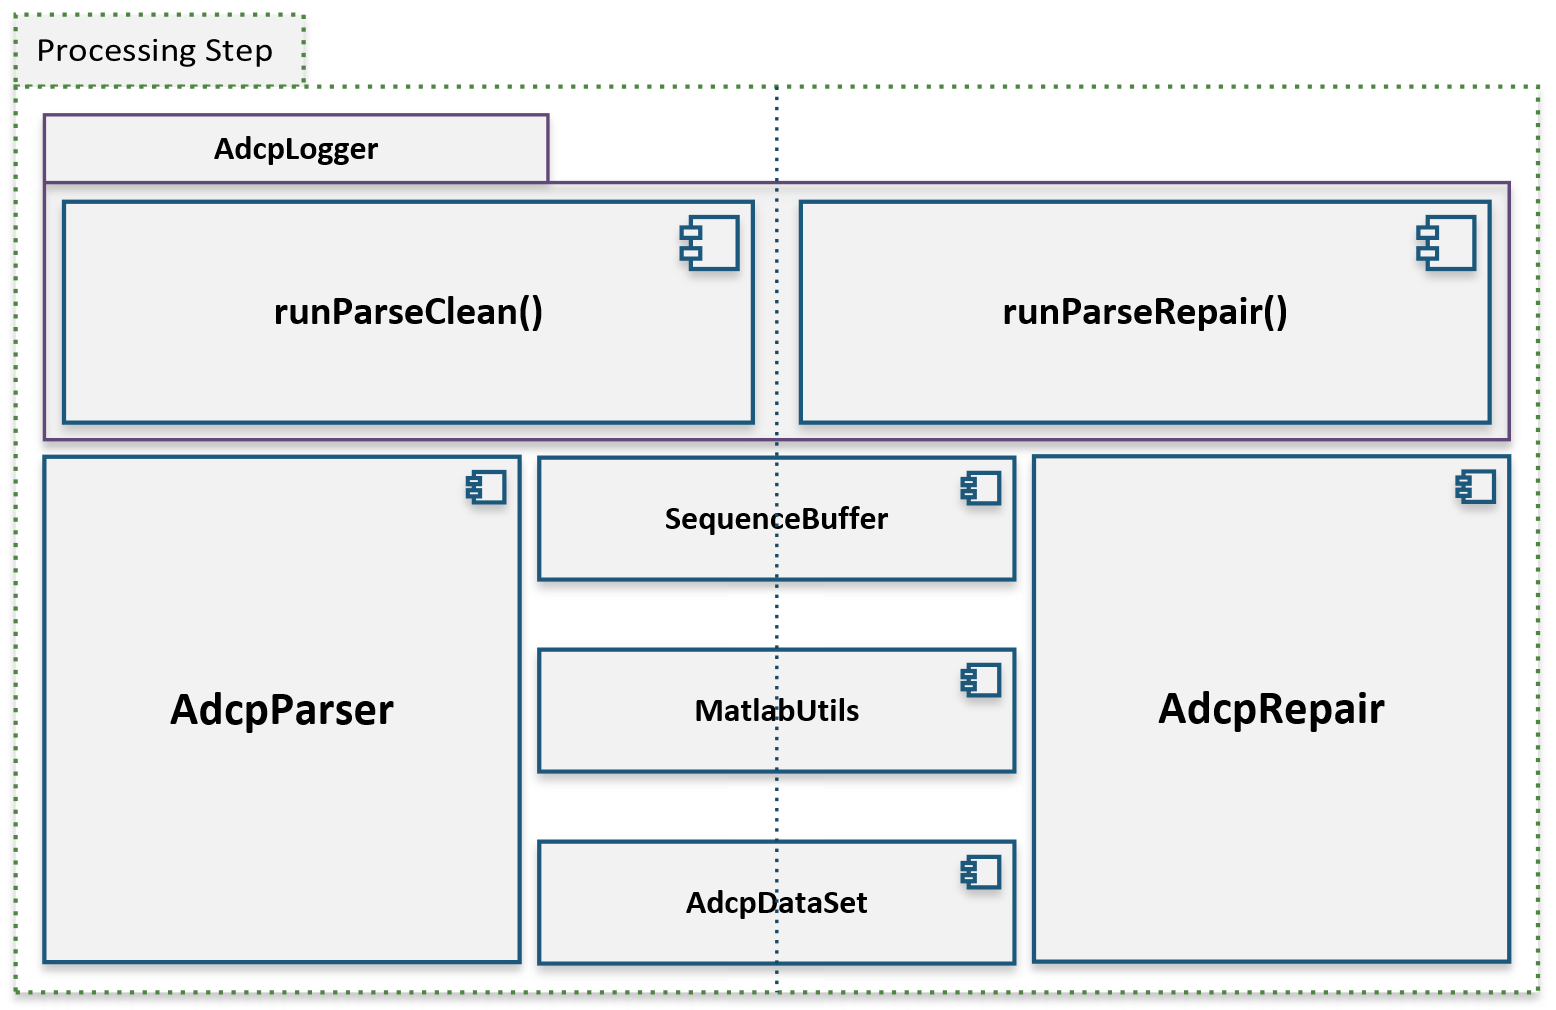
\includegraphics[width=0.8\textwidth]{components}
%        \caption{A component diagram over all components used in the ADCP logger class.} 
%\end{figure}

The output components for the \texttt{OutputThread} were again decided based on older use cases. Either \texttt{BinaryFileOutput} for one result file, e.g. to merge a month of burst data files into one file, or \texttt{BinaryFileListOutput} to generate a list of files based either on timestamps. The output components are message based, where a block of binary data is combined with a time stamp into a message. Thus it is possible to decouple the output from ADCP data structures and making it independent and usable for other sensor types, as long as the output is binary. 

In reflection on the requirements R8, R9, and R10 the resulting architecture is structured, decoupled and formed around components. The MATLAB component, the sequence buffer as well as the input-output components are completely independent of the ADCP context and would be ready to use for other projects.

The design of the data structures used in the application should also follow the guidelines formed by the requirements. 
\vspace{9em}

\begin{figure}[!ht]
\centering
      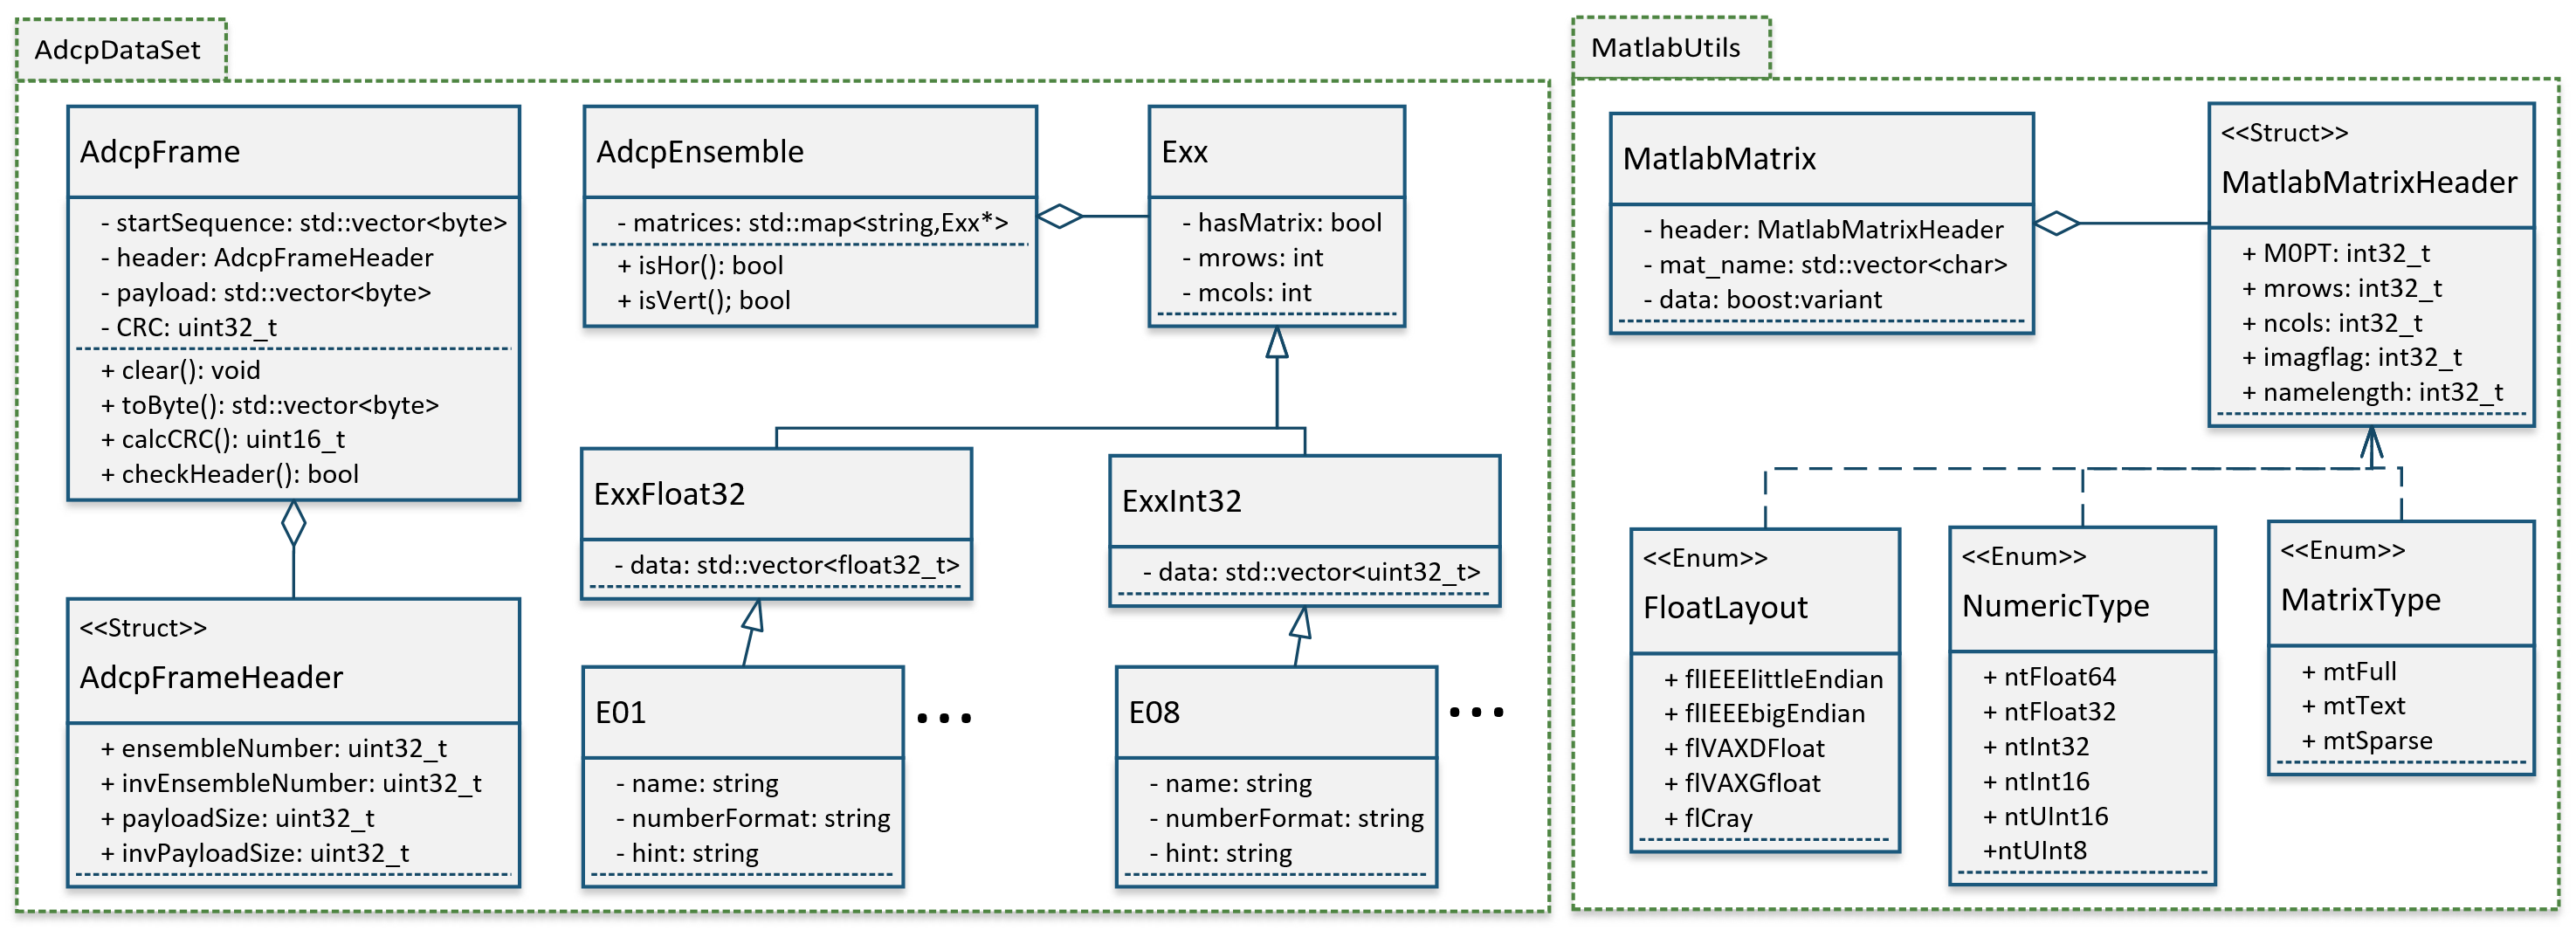
\includegraphics[width=1\textwidth]{data_structures}
        \caption{A class diagram representing the implemented data structures}
\end{figure}

Figure 3.3 shows an overview of the used classes. In this figure, a distinction of the modules was done by UML packets. Only one data structure uses inheritance, the ADCP ensemble with its matrix classes, in the other cases it was simply not necessary! The degree of inheritance was tested in various scenarios from a complete flat hierarchy to the final version over three layers. The reason why inheritance was necessary in the first place, were the two different data types used in the ADCP data matrices. The decision for the current final approach resulted in better usability working with base class pointers. It saves a lot of code lines if one is able to iterate over an array of base class pointers instead of writing the code ten or more times. This way it is also possible to instantiate a \texttt{AdcpEnsemble} without preallocated matrix classes, and add them only if needed. There were arguments against this approach, especially performance wise because the downcasts were expensive. As the development progressed it turned out that this was only a compiler setting. If the code was compiled for release, the compiler optimized as far as a concrete distinction between a high- or a low inheritance hierarchy was not detectable anymore.

\section{Implementations Specific Decisions}
For the development process, some decisions had to be taken. Important was the choice of the development environment. It was decided to develop on Windows and test the code on a small arm7 low-power device. To be able to use the same compiler on both architectures it was needed to use another integrated development environment (IDE) than the most famous C++ environment Visual Studio. The decision fell on CLion from JetBrains \cite{clion} a relatively new IDE with a lot functionality and identical usability than their already well known Java IDE IntelliJ \cite{intellij}. As compiler was GCC 4.9.2 chosen in conjuncture with MinGW 64 Bit from nuwen \cite{mingw}. The reason were the already integrated Boost libraries and the pre-installed CMake building tool.\\
The decision to work with the new C++11 \cite{cpp_11} instead of the old C++03 \cite{cpp_03} standard was quickly taken. It introduces a lot of new functionality, some of it crucial for efficiency (\texttt{std::move}), memory management (\texttt{std::shared\_ptr}) and threading (\texttt{std::atomic}). During the implementation period in early 2016 C++11 was already widespread and compatible compilers available for almost every platform. On the target platforms for the software, even C++14 \cite{cpp_14} was already available but in order to support GCC versions smaller than 4.9 for older Linux devices, only C++11 features were used.
\subsection{Library Decisions}
This sections will describe the choices that were made in the selection of used libraries described in Chapter 2.

The first library introduced was Boost \cite{boost}. When working with C++ and a portability requirement, one of the first libraries used is Boost. Boost is a collection of portable C++ source libraries covering a broad spectrum off applications. The libraries provide reference implementations that may be later included in the C++ standard. A large part of Boost was already included in the new C++11 Standard \cite{cpp_11} but not everything needed in this project. The decision to use Boost was quickly taken, mainly because the compiler in MingGW \cite{mingw} did not support the standardized \texttt{std::thread}, which was introduced in C++11 and thus leaving no other choice than Boost for portable threading. Otherwise the Boost.Asio library \cite{boost_asio} for network communication was also a driver to use Boost, it was used for the portable communication over serial ports. The used version 1.60.0 of Boost was at the time the newest, it was the first one where a lot of code was implemented in C++11 allowing e.g. the use of efficient move semantics.

With the inclusion of Boost the decision on other libraries was driven by its availability in Boost. It would make no sense to introduce other dependencies into the project if a solution was available in Boost. The following choice was influenced mostly by on the availability: Boost.Program\_Options, used to parse program parameters from an initialization (INI) file. This library was the only viable option, it was able to combine parameters from the command line as well as from a configuration file. Other options like getopt \cite{getop} or a beautiful small library TCLAP \cite{tclap} were only focused on the command line arguments. 

In the development process, two external components were included. The first one was a lock-free thread-safe concurrent queue developed by Cameron Desrochers \cite{moody}. He designed a Multi-Producer-Multi-Consumer (MPMC) queue with one of the fastest implementations e.g. compared to Boost's lock-free data structures. This queue was used as connection between threads, and with the help of explicit consumer- and producer tokens the queue was used as a Single-Producer-Single-Consumer (SPSC) queue. In the decisions which technology should be used to connect the threads the first consideration was the use of the C++ Standard Library (STL) \cite{stl_stream} input and output streams. The lack of thread-safety of most STL data structures and streams would have made this approach complicated as the synchronization of the threads would have been been needed to be done by hand. The queue developed by Cameron was the best choice to connect the threads and removed the need of manual thread management.\\
The second external code used, is just a beautiful implemented wrapper around the serial port class of Boost.Asio and was implemented by Terraneo Federico \cite{serport}. The reason to use this class was only a simplification of the development process, which allowed to set the focus on other parts of the project implementation.

For the sake of simplicity the following naming scheme for files with ADCP data was decided. The file extension is a point followed by three letters. Left of the extension follows a eight-digit number, which is again followed on the left side by a unspecified prefix as illustrated in Figure 3.4.
\begin{figure}[!ht]
$$ \underbrace{ADCP}_{\text{Prefix of variable length}}\underbrace{00000123}_{\text{Eight-digit number}}\underbrace{.bin}_{\text{Extension}}$$
        \caption{Naming scheme of ADCP files.}
\end{figure}


%-------------------------------
%-------------------------------
%-------------------------------
\chapter{Implementation}
This chapter gives detailed insights on implementation specific aspects of the project. In the first three sections, the standalone components without ADCP related dependencies are introduced, followed by a description of the parser class. The last section describes the resulting architecture of the main program. 
\section{MATLAB Component}
Section 2.2 described the data generated by an ADCP. It was shown that the payload of each ensemble is serialized in a MATLAB v.4 file format \cite{matlab}. This format is used by General Acoustics e.K. for other sensor types like a sub-bottom profiler. The high portability to reuse the code and algorithms related to the MATLAB v.4 format predestines for a clean, independent and self contained code. To ensure the required independence the MATLAB component was implemented and tested before the other components and the main program.\\
The implementation strongly followed the official MATLAB v.4. file structure documentation \cite{matlab}. The structure defined there has a lot more possible data types and matrix types than used by the ADCP. For example, in a MATLAB v.4 matrix the data may be stored as a sparse matrix, but this feature is not used for ADCP ensembles. The unused features were prepared but not implemented as seen in Listing 4.1.
\pagebreak
% prepared code snippet
\begin{lstlisting}[language=C++, caption=Code snippet of unimplemented logic]
        case NumericType::ntUInt16 : {
            //optional
        }
        case NumericType::ntUInt8 : {
            //optional
        }
    }
    return std::move(vec);
}
std::string MatlabWriter::reportMatrix(MatlabMatrix *matrix){
    //optional
}
\end{lstlisting}

The decision to skip the implementation of project unrelated parts helped focusing the programming efforts on other more complex parts of the project. The library is well structured and extendable, thus it will be a simple task to extend it if asked in forthcoming projects.

% matlab structure
\begin{figure}[ht]
\centering
      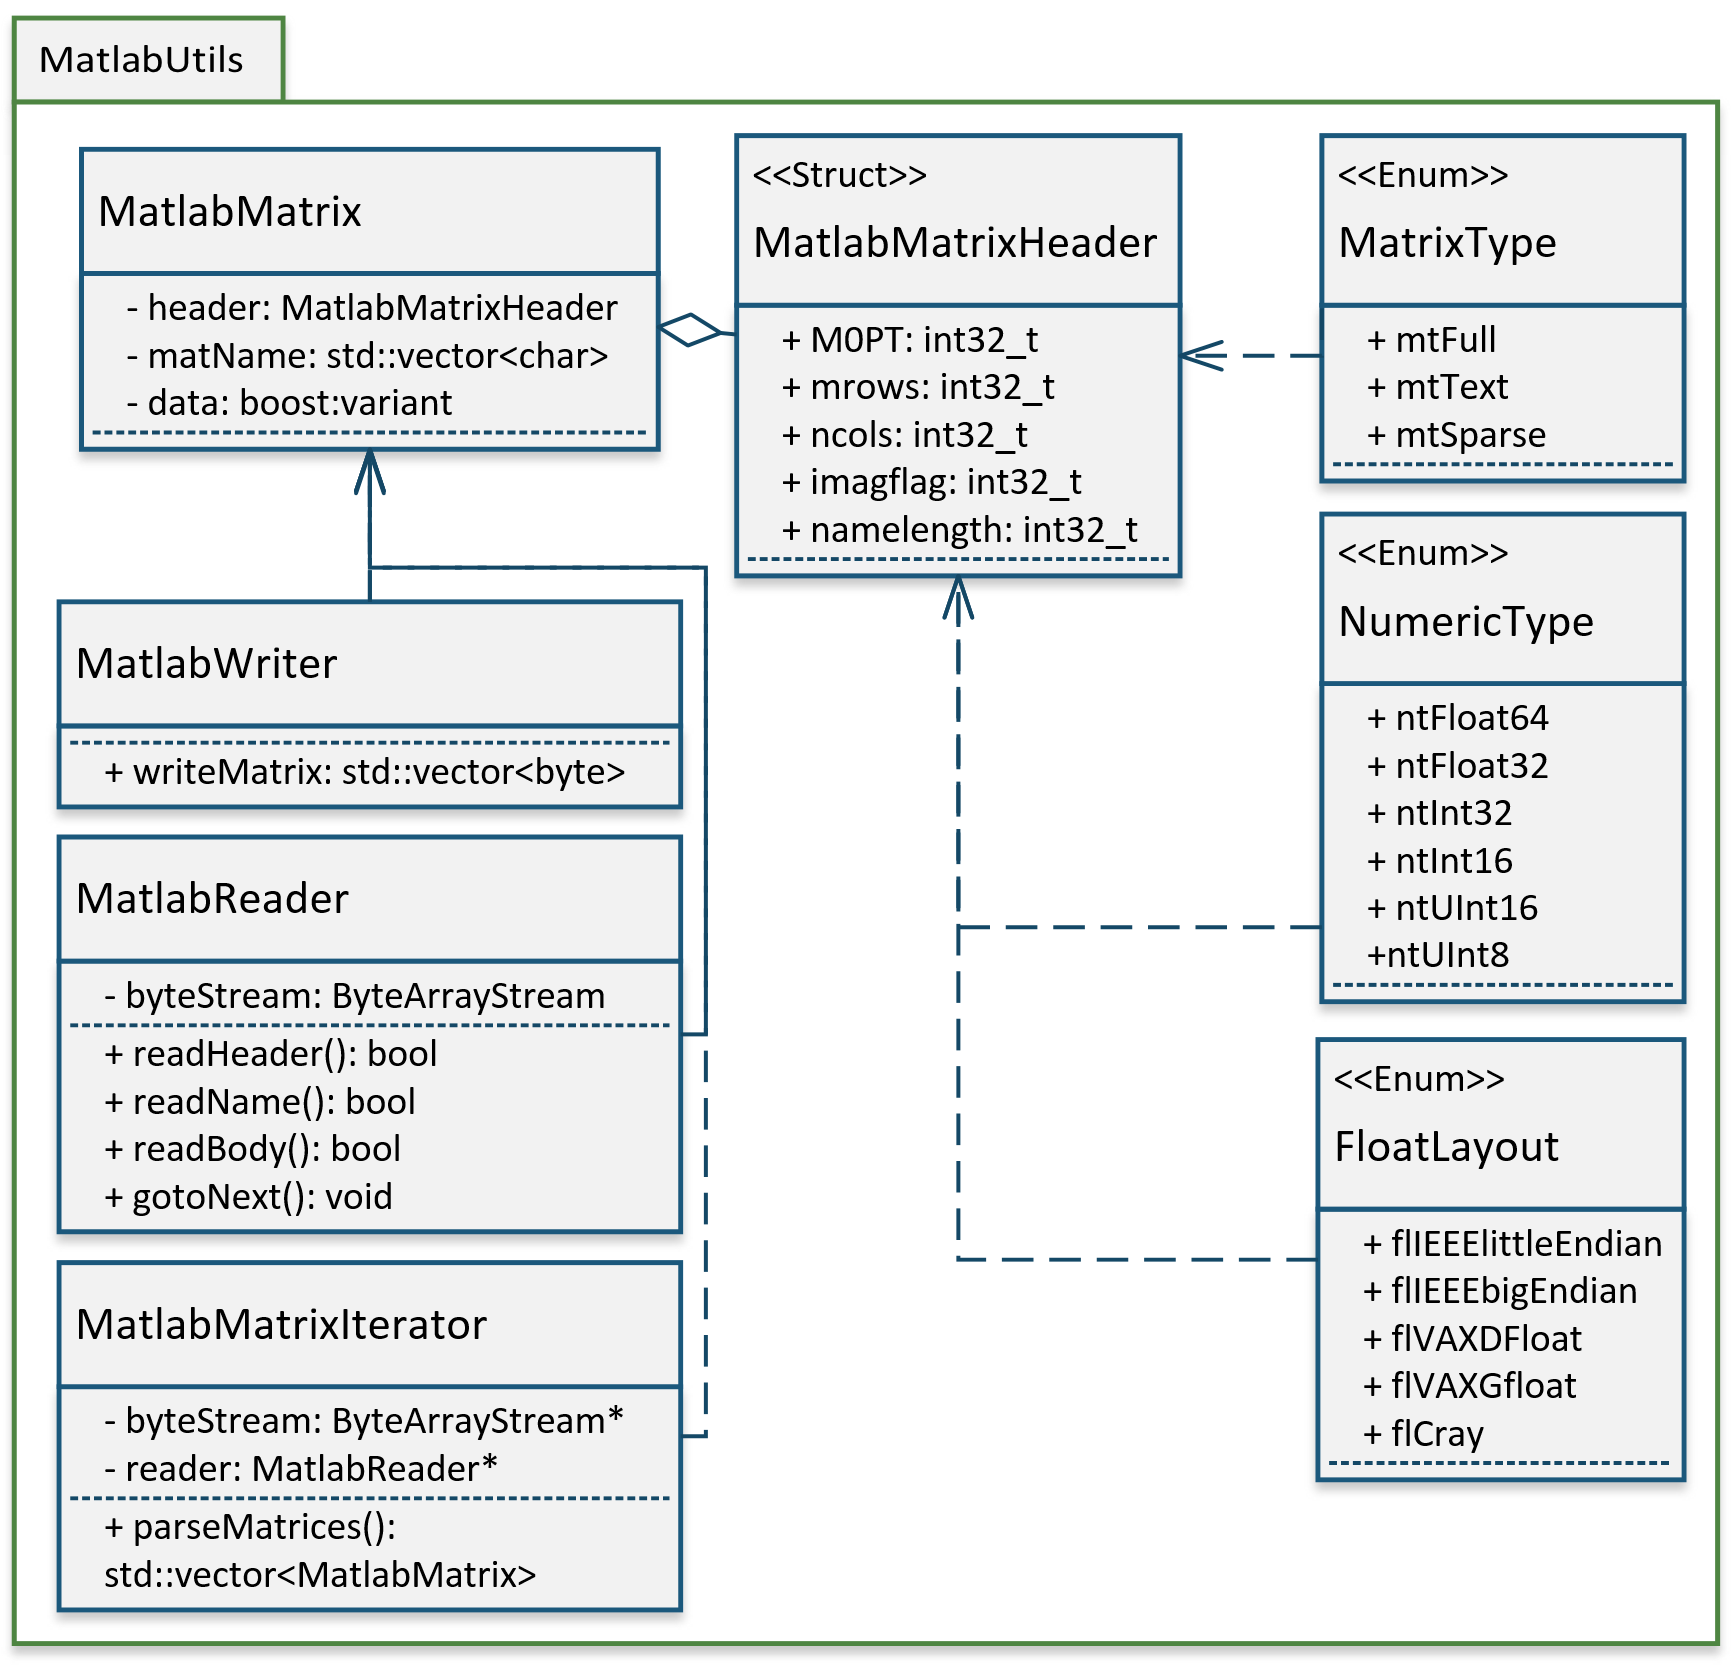
\includegraphics[width=0.8\textwidth]{mlab}
        \caption{A class diagram as overview of the MATLAB component.}
\end{figure}

The structure of the component is presented in Figure 4.1. The \texttt{MatlabMatrix} is the core class of the MATLAB component and stores a MATLAB matrix, the other classes, \texttt{MatlabReader}, \texttt{MatlabWriter}, and \texttt{MatlabMatrixIterator} are used to serialize and de-serialize these matrices. The \texttt{MatlabMatrix} class is described in the next subsection.
\subsection{MATLAB matrix Data Structure}
As presented in Figure 4.1 a \texttt{MatlabMatrix} contains a \texttt{MatlabMatrixHeader}. The header contains five \texttt{uint32} integers specifying the rest of the matrix and is implemented as a struct. The first integer, also called \texttt{M0PT}, is composed out of three other integers. The value is calculated as follows:
$$M\cdot1000 + 0 \cdot 100 + P\cdot 10 + T$$
$M$ represents the float layout, which specifies how the float is stored in bytes. Only little and big endian were considered for this project. $P$ is the numerical type of the matrix content and $T$ is the matrix type, which holds if the matrix is either a full matrix, sparse matrix or a matrix containing text. All three values are implemented as enums, their implementation is shown in Listing 4.2.
\vspace{1em}
\begin{lstlisting}[language=C++, caption=A code snippet showing the used enums and structs in the MATLAB header.]
struct  MatlabMatrixHeader {// Fixed 20 Byte matrix header
    int32_t M0PT;  			//  == FloatLayout * 1000 + NumericType * 10 + MatrixType
    int32_t mrows;
    int32_t ncols;
    int32_t imagflag;   	//  1 if matrix has imaginary part
    int32_t namelength; }; 	// 1 + name length

enum class FloatLayout {  	// equals M of M0PT in MatlabMatrixHeader
    flIEEElittleendian,
    flIEEEbigendian,
    flVAXDfloat,
    flVAXGfloat,
    flCray };
							// 0 of M0PT is always 0
enum class NumericType { 	// equals P value of M0PT in MatlabMatrixHeader
    ntFloat64,
    ntFloat32,
    ntInt32,
    ntInt16,
    ntUInt16,
    ntUInt8 };

enum class MatrixType {  	// equals T Value in MatlabMatrixHeader
    mtFull,
    mtText,
    mtSparse};
\end{lstlisting}
\pagebreak
The next two integers in the header after the \texttt{M0PT} value contain the number of rows and columns in the matrix. Next follows a flag if the matrix has an imaginary part, which would double the amount of data used. The last integer of the header contains the number of characters from the matrix name incremented by one to account for the string termination character.

The \texttt{MatlabMatrix} class additionally contains a vector of \texttt{char}'s to store the matrix name, in Figure 4.1 described as \texttt{matName}.\\
The matrix data is stored in a templated \texttt{boost::variant} vector to allow a range of data types for the data. The fairly complicated templating (Listing 4.3) needed to achieve this goal was taken from a great answer at Stackoverflow \cite{stackof}, With this solution the cumbersome inheritance hierarchy could have been bypassed. 
\vspace{1em}
\begin{lstlisting}[language=C++, caption=A code snippet showing the templating to allow various types in a Boost variant.]
template<class...>struct types {};
using matlab_types = types<int16_t, int32_t, boost::float32_t, boost::float64_t, uint8_t, uint16_t>;

namespace details {
    template<class types, template<class...>class target>
    struct apply_types {};
    template<class...Ts, template<class...>class target>
    struct apply_types<types<Ts...>, target> {
        using type = target<Ts...>;
    };
}
template<class types, template<class...>class target>
using apply_types = typename details::apply_types<types, target>::type;
...
// and used for a vector with variable types:
...

template<class...Ts>
using data_t = boost::variant< std::vector<Ts>... >;
apply_types<matlab_types, data_t> real;
\end{lstlisting}

%-------------------------------
%-------------------------------
\section{Sequence Buffer}
The idea of the sequence buffer has its origin at General Acoustics e.K. It serves as a buffer between binary input streams or input queues and a consumer. Figure 4.2 presents the simple API as a class diagram. The buffer can be used if the \texttt{read()} operations should be done in a all-or-nothing way. The buffer has a \texttt{find()} method that searches for a sequence in the current buffer. The buffer has three properties that define how the buffer mechanism works:
\pagebreak
\begin{itemize}
	\item The buffer can be hungry when \texttt{isHungry} is \texttt{true}, with this property on each \texttt{load()} operation it will load the maximal number of bytes that can be filled into the buffer. 
	\item If the second property \texttt{isAngry} is \texttt{true} the buffer throws an exception when the \texttt{find()} method fails and the buffer is full. 
	\item The third option \texttt{isAutodiscard} states if, in case of a \texttt{find()} failure the buffer should drop bytes to prevent a deadlock.
\end{itemize}
The set combination of these properties in conjunction with the preset buffer size should be considered carefully. If the byte sequence, which should be found, is longer than the maximal buffer size the \texttt{find()} method will always report \texttt{false} and the application ends in a deadlock. The same thing can happen if the buffer is neither \texttt{isAngry} nor on \texttt{isAutodiscard}. In these cases the application has to prevent the deadlock.\\
The maximum buffer size is set at instantiation, but extends itself based on the size of the requested \texttt{read()} and thus make sure that the buffer has enough space for a read.\\
The implementation was done specifically for the Moodycamel concurrent queue \cite{moody}. Other sources can easily be added for different projects. The buffer could also be extended to support \texttt{readLine()} operations on \texttt{CRLF} delimitered data. The stubs are already prepared. 
\begin{figure}[ht]
\centering
      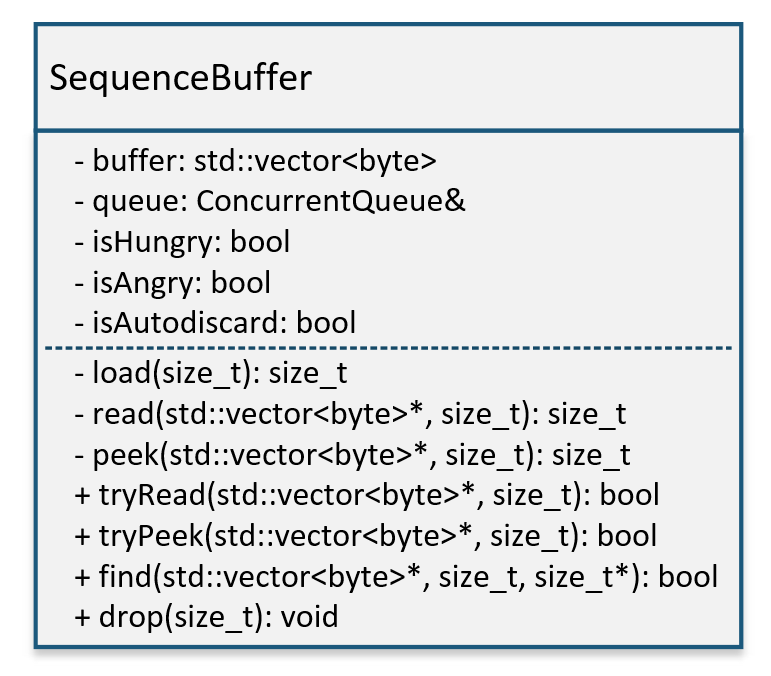
\includegraphics[width=0.7\textwidth]{seqbuf}
        \caption{A class diagram of the sequence buffer.}
\end{figure}

%-------------------------------
%-------------------------------
\section{ADCP Logger}
The heart of this software project was the implementation of the ADCP logger application. It integrates the separately developed components and forms the main program. This section shows the result of the implementation, explaining the architecture and specific technical specialties in a detailed top down approach.\\
As specified in the design decisions in Section 3.2, the architecture was implemented in a pipelined input-processing-output way. The program allows the execution of different components for each pipeline step. A configuration file is used to tell the program which component should be instantiated. The Boost.Program\_Options library was used to parse the configuration file and set all required parameters, it conveniently allows to check for invalid parameters and produces nicely formatted help output. Listing 4.4 shows an example of a configuration file, it describes how the most important settings of the application are set. The three modes \texttt{inputmode}, \texttt{processmode}, and \texttt{outputmode} define which component is used at runtime. The \texttt{inputpath} and the \texttt{outputpath} are used to tell the application where the input files are located, respectively where it should output new files. In case \texttt{serial} is chosen as \texttt{inputmode}, the comport \texttt{com} and the Baud rate \texttt{baudrate} have to be specified. 
\vspace{1em}
\begin{lstlisting}[language={Ini}, caption=A snippet of a configuration file for the ADCP logger application.]
                                        #       CONFIGURATION FILE      #
                                        #               for             #
                                        #          ADCP Logger          #
                                        #              v0.9             #
                                        #-------------------------------#
# Possible Input drivers:
#           - serial: serial input
#           - file: prozesses a single file
#           - filelist: processes a continoues list of files in folder
inputmode=filelist

# Possible Process Components:
#           - repair: trys to recover as much as possible
#           - clean: removes all unnecessary data
processmode=clean
# Possible Output drivers:
#           - file: prozesses a single file
#           - filelist: processes a continoues list of files in folder
outputmode=file
# Input path to a file
inputpath=C:\TEMP\output\ADCP00000020.bin
# Output path to a directory
outputpath=C:\TEMP\output
[input]
com=COM7
baud=19200
\end{lstlisting}
\pagebreak
Each pipeline step is implemented as a thread. All threads are connected over Moodycamels lock-free concurrent queues \cite{moody}. The queues are set up as SPSC queues and use explicit producer and consumer tokens to maximize performance. Listing 4.5 shows how the token is used to dequeue elements from an input queue. In line one, the consumer token is created for the incoming data queue. In line four an element is dequeued from the queue with help of the consumer token.
\vspace{1em}
\begin{lstlisting}[language=C++, caption=Code snippet showing the use of consumer tokens.]
moodycamel::ConsumerToken ct(istream);
while(!exit){
    BinaryMessage msg;
    if(istream.try_dequeue(ct,msg)) {
...
\end{lstlisting}

The threads run concurrently until the end of the execution. Each thread exits if its predecessor is finished. If this is the case, the thread synchronizes with its predecessor over an atomic boolean value. It is important that the memory state of the predecessor gets propagated to the thread receiving the exit signal. The implementation of the memory propagation was done with the new C++11 \texttt{std::atomic\char`_thread\char`_fence} memory barriers. This step was needed that the thread determined to exit, can reliably see if its input queue is empty. The critical function here is the \texttt{moodycamel::size\char`_approx()} function. It only returns the correct size of the queue if the memory effects of the enqueue operations in the predecessor threads have propagated. With the use of the described memory fences this state can be reliably provided. How this was implemented is shown in Listing 4.6.
\vspace{1em}
\begin{lstlisting}[language=C++, caption=Code snippet highlighting the memory barriers.]
// previous thread is finished, and queue is empty, then exit thread
if (exit->getPrevious()->load(std::memory_order_relaxed)) {
    // make sure the memory effects have propagated before checking the size
    atomic_thread_fence(std::memory_order_acquire);
    // look if the input queue is empty
    if (istream.size_approx() <= 0) {
        // if it is empty, set memory fence for next thread
        atomic_thread_fence(std::memory_order_release);
        exit->getCurrent()->store(true, std::memory_order_relaxed);
        exitLoop = true;
    }
}
\end{lstlisting}

The component selection based on the configuration file (Listing 4.4) is done in the main function of the program through simple if-else statements. Depending on the selected modes the according thread function is executed. This architecture allows to insert either more components to select at each step (e.g. a third processing component) or extend the model with a reasonable number of new steps implemented as additional threads e.g. a wave processing step, which calculates wave informations based on the parsed data. 

The next three sections look at the currently implemented steps of the processing pipeline. A class diagram is presented for each step. The diagrams omit getter and setter methods as well as constructors to simplify the diagram. If a component was already shown before, it is only added as a simplified package to save space. In the implementation, byte conversion functions and time functions were used in all components. They were implemented in namespaces in the \texttt{ByteUtils.h} and \texttt{TimeUtils.h}, their functionality is simple and commonly used.
\subsection{Input Step}
In Section 3.2 an overview of the input components was described. The following class diagram (Figure 4.3) shows the three input components \texttt{SerialInput}, \texttt{BinaryFileInput} and \texttt{BinaryFileListInput}. All three classes are derived from the abstract class \texttt{BinaryInput} and depend on Moodycamel concurrent queue \texttt{ConcurrentQueue}. The classes are located in the file \texttt{BinaryIO.h} together with the output classes.

\begin{figure}[ht]
\centering
      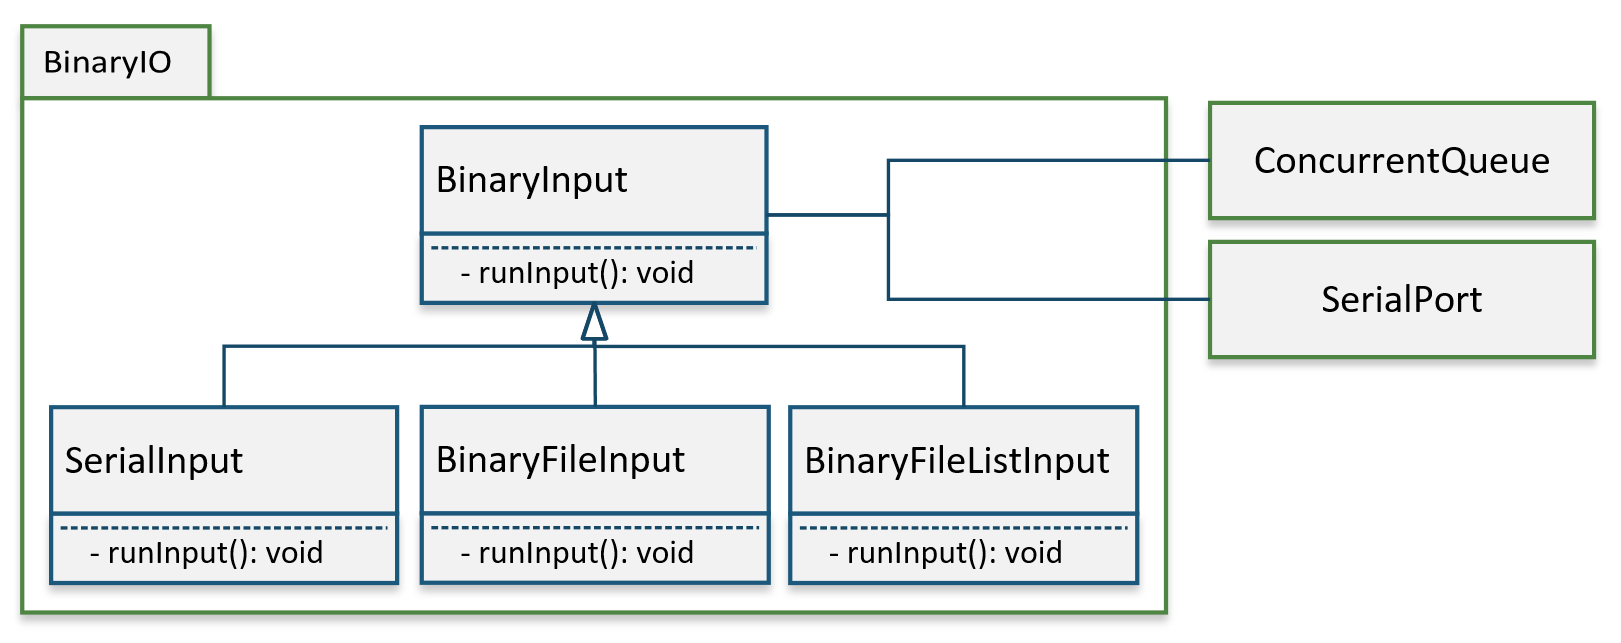
\includegraphics[width=0.95\textwidth]{input}
        \caption{A class diagram of the input components}
\end{figure}

The classes have only the \texttt{runInput()} method where the business logic of the component was implemented. One of these functions will be executed by the input thread. \\ 
The \texttt{SerialInput} class simply polls a serial port regularly with the help of the \texttt{SerialPort} class, and tries to enqueue the data to the queue, if it is not able to enqueue, it buffers the data in a vector and tries it again in the next loop. If the buffer exceeds its maximum size, old data is thrown away. With proper parametrization of the queue- and buffer sizes depending on the host machine this should never be the case!\\
The \texttt{BinaryFileInput} class is used to process one file. It first checks the availability of the file and calculates the file size as number of bytes. Depending on that size, either the whole file is enqueued at once, or it is enqueued in chunks. Once again one has to be careful to set the parameters correctly or else the application ends up  in a deadlock.\\
The \texttt{BinaryFileListInput} class does essentially the same thing as the \texttt{BinaryFileInput} but iterates over a directory and processes all files that follow the naming scheme defined in Section 3.3 and have a number bigger than the starting file.
\subsection{Processing Step}
The processing step contains most of the business logic implemented in this project. Figure 4.4 presents the class structure used for this step. The MATLAB component as well as the sequence buffer were presented in Section 4.1 and 4.2 and are only included as packets.

In the center is the \texttt{AdcpLogger} class. It has two methods \texttt{runParseClean()} and \texttt{runParseRepair()}. These two methods can be seen as the two processing components shown in the component overview in Section 3.3. One of them gets executed in the processing thread.

The \texttt{runParseClean()} method satisfies the requirement to parse the incoming ADCP data and throw away the unused parts. It uses the \texttt{SequenceBuffer} class to buffer the incoming binary data from the input queue. The \texttt{AdcpParser} class is then used to extract complete \texttt{AdcpFrames} from the buffer.

The parser itself is a small finite state machine shown in Figure 4.5. It is divided into four states. If the parser enters a new state, the code belonging to this step is executed, depending on the result it can enter into a new state or has to run the state code again in the next iteration. The first state is \texttt{StartSequence}. In this state the parser uses the \texttt{find()} function of the sequence buffer to find the ADCP start sequence in the input queue. If successful, the parser transitions to the second state \texttt{Header} and reads the ADCP header. If the header is invalid the frame will be discarded and the parser is reset to the \texttt{StartSequence}. When a correct header is found the parser jumps to state three \texttt{Payload} and reads the number of bytes specified in the header into the frame payload. In this step the parser transitions always to the last state \texttt{CRC} where it reads the target CRC value from the stream and compares it to the actual CRC calculated from the previously read payload. Depending on the result the frame is either thrown away when the CRC's are not equal, or it is made available for collection. If in either one of the states the sequence buffer can not deliver because its queue is empty, the parser remains in the same state.

With this behavior of the parser the \texttt{runParseClean()} method is guaranteed to always get complete frames. The payload of these frames is then processed with help from the \texttt{MatlabUtils} component to extract the MATLAB matrices which then are filled into an ensemble. At this step the cleaning happens. The ensemble is only filled with matrices needed for the further processing by General Acoustics e.K. At the moment the matrices E000001 or E000003 and E000008, E000009, E000015 are kept.

The ensembles are then converted back to an ADCP frame and then into a byte sequence. The byte sequence is then packed into a binary output message together with the time stamp from the ensemble. The message is then enqueued to the output queue, available for the output step.

\pagebreak

\begin{figure}[!ht]
\centering
      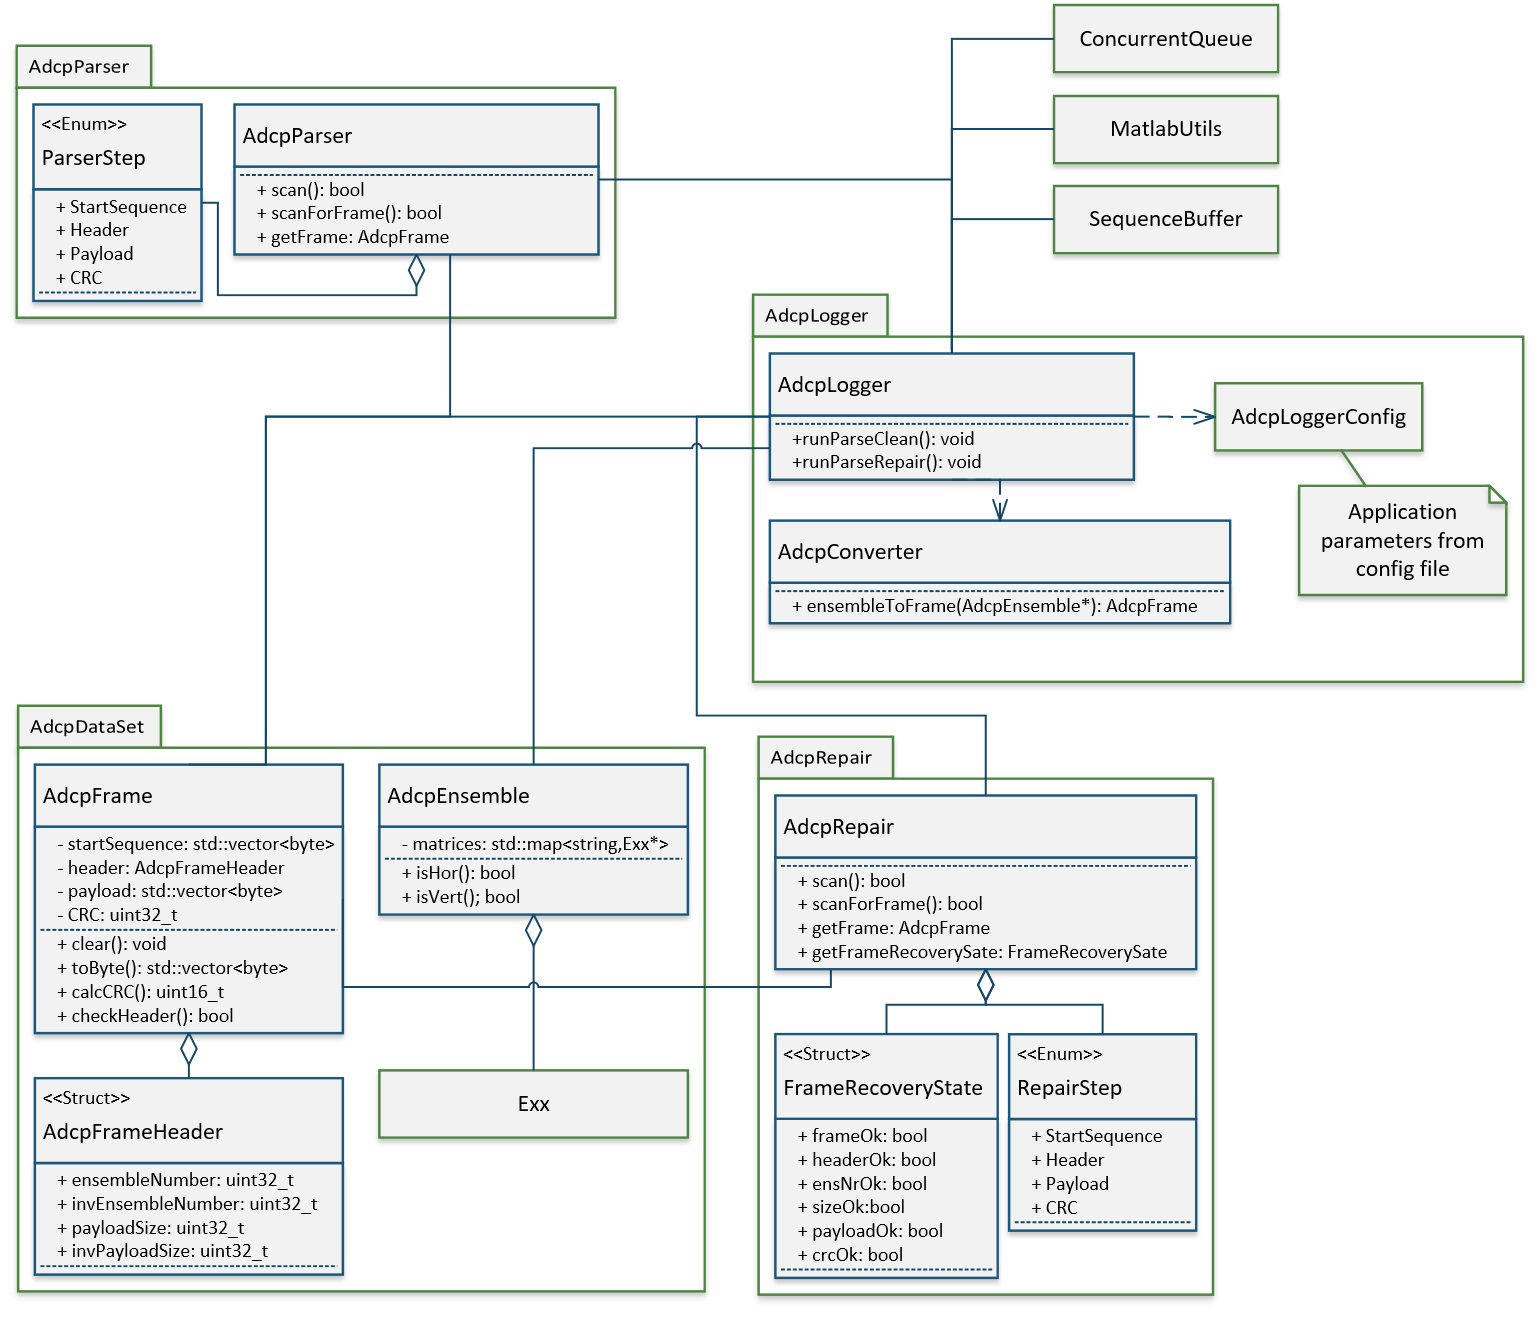
\includegraphics[width=1.05\textwidth]{logger_class}
        \caption{A class diagram of the components used for the processing step}
\end{figure}
\vspace{4em}

\begin{figure}[ht]
\centering
      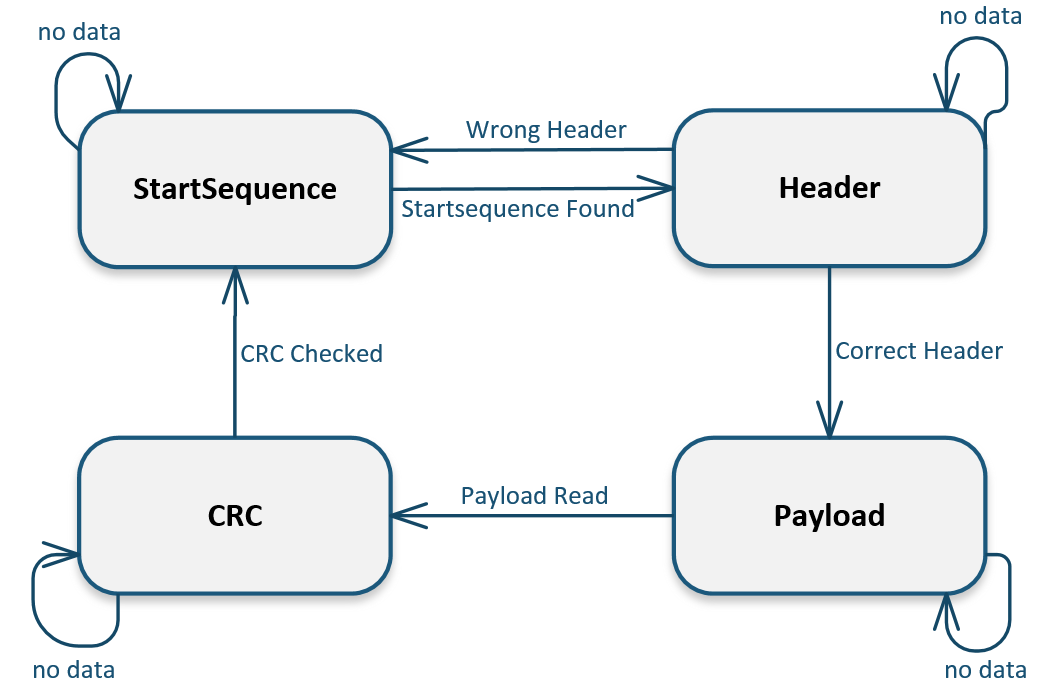
\includegraphics[width=0.7\textwidth]{parser}
        \caption{A state diagram of the ADCP parser}
\end{figure}
\begin{figure}[!hb]
\centering
      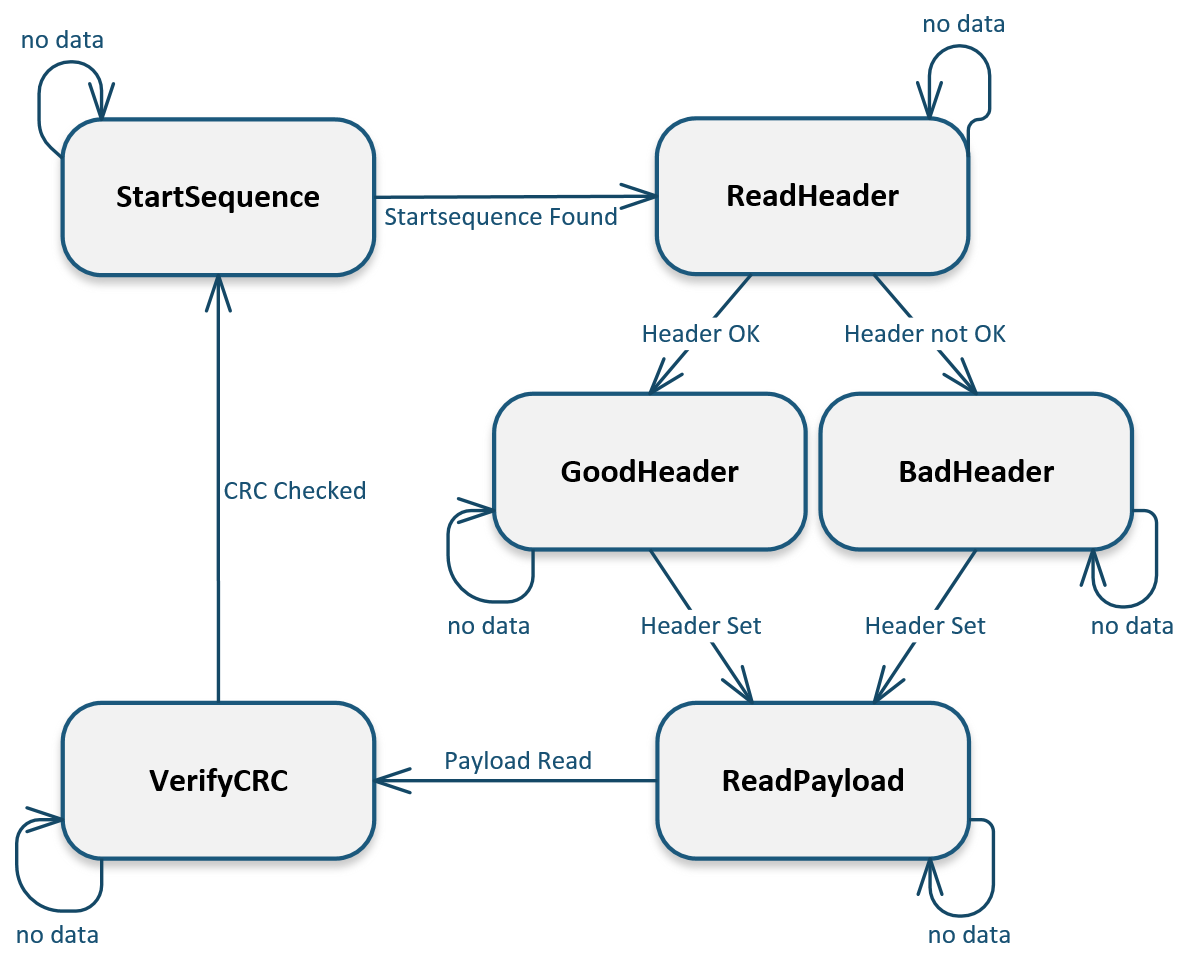
\includegraphics[width=0.7\textwidth]{repair}
        \caption{A state diagram of the ADCP repair parser}
\end{figure}
\pagebreak
The \texttt{runParseRepair()} component was introduced as a result from an urgent request from General Acoustics e.K.. It was needed to repair and save as much ADCP data as possible from corrupted files. The problem was a defective communication between an ADCP and the data logger. The data stream lost bytes fairly regularly.\\
The task turned out to be much more complicated than thought at first. A lot of assumptions had to be taken, e.g. only frames with a complete start sequence were considered. Another preset constraint was the number of bytes that were allowed to miss in each matrix. 

The result of considering various error scenarios was a new parser class, the \texttt{AdcpRepair}. It is also a state machine but is also able to extract also ensembles containing errors. The data to be extracted has to be at least more or less recognizable as an ADCP frame to be able to reconstruct it. Figure 4.6 shows the state machine of this parser.

In the \texttt{runParseRepair()} method the received frames are processed in the expectation to recover as much data as possible. Probably the most important correction happens at the moment where the byte stream is converted to integers or floats. If a byte is missing the generated number is semantically wrong or even not considered as a number. Listing 4.7 shows the code snippet that tries to find where the byte is missing, and searches for the next possible healthy value. First the number of missing bytes is evaluated, if it is smaller than the number of bytes allowed to miss, every four bytes in the binary vector are converted to an integer, and semantically checked if the result makes sense. If not, the resulting value is set to -999 to indicate an error. After an error is found, the algorithm iterates over the next four bytes, always moving forward one byte, and checking if the converted value makes sense. After the interleaved for loop has finished, all bytes from the input are either semantically correct values, or replaced by -999.\\
After recovering as much as possible, all data like the time stamp or the ensemble number are tested again for plausibility, if everything seems fine the frame is converted to a message and enqueued ready for the output thread.

This algorithm only works reliable if the number of missing bytes is not too high, while testing the algorithm a maximum of 2 missing bytes per float matrix delivers acceptable results. It also has room of improvement but it was not a core requirement of this project. Originally only 20 out of 2048 ensembles were healthy, with this function the number could be raised to over 800 which was enough for further wave analysis.
\vspace{20em}
\pagebreak

\begin{lstlisting}[language=C++, caption=Code snippet from the repair function finding missing bytes.]
size_t expectedSize = bins*beans* sizeof(boost::float32_t);
size_t realSize = (posE4 - 5 * sizeof(int32_t)) - posE3;
double difference = expectedSize-realSize;
// only at most maxBytesLost bytes lost - to many bytes are not considered
if(difference >= 0  && difference <= maxBytesLost){
    boost::float32_t res;
    int offset = 0;
    for(int i = 0; i < bins * beans; i++) {
        auto vecbuf = std::vector<unsigned char >(posE3 + offset + i * 4, posE3 + offset + i * 4 + 4);
        res = ByteUtils::byteVecToFloat32(vecbuf, ByteUtils::Endianness::LittleEndian);
        //bad - check for nan
        if(res < -15.0f || res > 15.0f || (res > 0.00f - epsilon && res < 0.00f + epsilon) || res != res) {
            e3.push_back(-999.0f);
            if( i < bins*beans -1){
                i++;
                //try to find next healty value
                for(int j = -3; j <= 0; j++){
                    vecbuf = std::vector<unsigned char >(posE3 + offset + j + i * 4, posE3 + offset + j + i * 4 + 4);
                    res = ByteUtils::byteVecToFloat32(vecbuf, ByteUtils::Endianness::LittleEndian);
                    if((res > -15.0 || res < 15.0) && (res < 0.00f - epsilon || res > 0.00f + epsilon)){
                        offset += j;
                        e3.push_back(res);
                        break;
                    }else{
                        if(j == 0){
                            e3.push_back(-999.0f);
                        }
                    }
                }
            }

        }else{ //good
            e3.push_back(res);
        }
    }
}
\end{lstlisting}

\pagebreak

\subsection{Output Step}
The output step is very similar to the input step. The class diagram in Figure 4.7 shows the two output components \texttt{BinaryFileOutput} and \texttt{BinaryFileListOutput} as specified in the design decisions. The classes are derived from the abstract class \texttt{BinaryOutput} and are located in the file \texttt{BinaryIO.h} together with the input classes.

\vspace{3em}
\begin{figure}[!ht]
\centering
      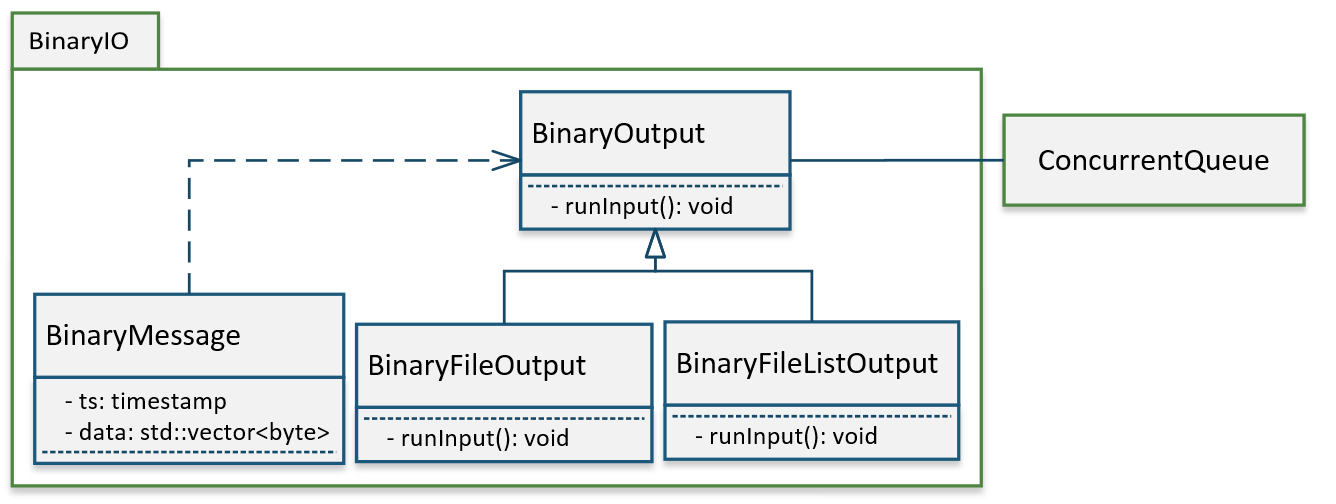
\includegraphics[width=0.95\textwidth]{output}
        \caption{A class diagram of the output components}
\end{figure}
\vspace{3em}

Similar to the input components, the classes have only the \texttt{runOutput()} method where the business logic of the component was implemented. One of these functions will then be executed by the output thread. Both classes take their input data from a Moodycamel concurrent queue in form of a message. A message has a time stamp and a vector of bytes. The message class is also located in the \texttt{BinaryIO.h} file together with the output components. In this application a message consists of the data of one ensemble.

The \texttt{BinaryFileOutput} class is used to store all incoming messages in a single file. The \texttt{BinaryFileListOutput} class generates a list of files. The decision if a new file is opened depends on the times-tamp of the message and a preset interval. One could store an entire day in a file, or only a burst of 10 minutes. In real-time operation it makes sense to open new files burst-wise all 10 minutes.